\documentclass[preprint]{sigplanconf}

%include agda.fmt
%include main.fmt
% Packages
\usepackage{amsmath}%
\usepackage{tikz}%
\usepackage{tikz-qtree}%
\usepackage{subfigure}%
\usetikzlibrary{arrows,positioning}%
\usepackage{listings}%
\usepackage{url}%
\usepackage{wasysym}%

% Unicode support
\usepackage{textgreek}
\usepackage{ucs}
\usepackage[utf8x]{inputenc}

\DeclareUnicodeCharacter{948}{\ensuremath{\delta}}
\DeclareUnicodeCharacter{955}{\ensuremath{\lambda}}

% Coloured comments
\usepackage{color}
\usepackage{ifthen}
\newboolean{showNotes}
\newboolean{marginNotes}
\setboolean{showNotes}{false}
\setboolean{marginNotes}{false}
\newcommand{\marginNote}[1]{
\ifthenelse
  {\boolean{marginNotes}}
  {\marginpar{#1}}
  {#1}}

\newcommand{\todo}[1]{
\ifthenelse
  {\boolean{showNotes}}
  {\marginNote{\textcolor{red}{\textbf{Todo:~}#1}}}
  {}}

\newcommand{\wouter}[1]{
\ifthenelse
  {\boolean{showNotes}}
  {\marginNote{\textcolor{blue}{\textbf{Wouter:~}#1}}}
  {}}

\newcommand{\pepijn}[1]{
\ifthenelse
  {\boolean{showNotes}}
  {\marginNote{\textcolor{blue}{\textbf{Pepijn:~}#1}}}
  {}}


\begin{document}

\conferenceinfo{ICFP'14} {September 1--3, 2014, G\"oteborg, Sweden}

\title{Auto in Agda}
\subtitle{Programming proof search}

\authorinfo{Pepijn Kokke \and Wouter Swierstra}
           {Universiteit Utrecht}
           {pepijn.kokke@@gmail.com \quad w.s.swierstra@@uu.nl}

\maketitle

\begin{abstract}
  Proof automation is important. Custom tactic languages are hacky. We
  show how proof automation can be programmed in a general purpose
  dependently typed programming language using reflection. This makes
  it easier to automate, debug, and test proof automation.\todo{Write
    good abstract}
\end{abstract}

\section{Introduction}
\label{sec:intro}

Writing proof terms in type theory is hard and often tedious.
Interactive proof assistants based on type theory, such as
Agda~\cite{agda} or Coq~\cite{coq}, take very different approaches to
facilitating this process.

The Coq proof assistant has two distinct language fragments. Besides
the programming language Gallina, there is a separate tactic language
for writing and programming proof scripts. Together with several
highly customizable tactics, the tactic language Ltac can provide
powerful proof automation~\cite{chlipala}. Having to introduce a
separate tactic language, however, seems at odds with the spirit of
type theory, where a single language is used for both proof and
computation.  Having a separate language for programming proofs has
its drawbacks. Programmers need to learn another language to automate
proofs. Debugging Ltac programs can be difficult and the resulting
proof automation may be inefficient~\cite{brabaint}.

Agda does not have Coq's segregation of proof and programming
language.  Instead, programmers are encouraged to automate proofs by
writing their own solvers~\cite{ulf-tphols}. In combination with
Agda's reflection mechanism~\cite{van-der-walt}, developers can write
powerful automatic decision procedures~\cite{allais}. Unfortunately,
not all proofs are easily automated in this fashion. When this is the
case, the user is forced to interact with the integrated development
environment and manually construct a proof term step by step.

This paper tries to combine the best of both worlds by implementing
a library for proof search \emph{within} Agda itself. More specifically,
this paper makes the following novel contributions:

\begin{itemize}
\item %
  After illustrating the usage of our library with several motivating
  examples (Section~\ref{sec:motivation}), we show how to implement a
  Prolog interpreter in the style of \citet{stutterheim} in Agda
  (Section~\ref{sec:prolog}). Note that, in contrast to Agda,
  resolving a Prolog query need not terminate. Using coinduction,
  however, we can write an interpreter for Prolog that is \emph{total}.
\item %
  Resolving a Prolog query results in a substitution that, when applied
  to the goal, produces a term that can be derived from the given
  rules. We extend our interpreter to produce a proof term that
  witnesses the validity of the resulting substitution
  (Section~\ref{sec:proofs}).
\item %
  We integrate this proof search algorithm with Agda's
  \emph{reflection} mechanism (Section~\ref{sec:reflection}). This
  enables us to \emph{quote} the type of a lemma we would like to
  prove, pass this term as the goal of our proof search algorithm, and
  finally, \emph{unquote} the resulting proof term, thereby proving
  the desired lemma.
\item %
  \wouter{Example? Can we use our proof search to find out why a proof
  is not being found automatically?} \pepijn{I don't see how you would
  envision this---all we can say is ``No, all combinations of up to $d$
  of your hints fail to produce anything meaningful''---which, I suppose
  is not what you're after.}\wouter{I mean: add a 'debugging' mode to the
  auto function, giving some trace information about the search. This can
  help figure out that we are missing a certain lemma -- this is harder to
  see in Coq using auto. See the debug trace described here
  \url{http://adam.chlipala.net/cpdt/html/LogicProg.html}}
  \pepijn{Hmm. Dat moet te doen zijn. Lijkt me wel iets wat buiten de
    scope van dit project valt, voor nu. Het zal in ieder geval wat
    werk zijn.}\wouter{Laten we ons eerst richten op dit paper schrijven;
    mochten we tijd over hebben, kunnen we altijd naar dit soort dingen
    kijken.}
\end{itemize}

All the code described in this paper is freely available from
GitHub\footnote{
  See \url{https://github.com/pepijnkokke/AutoInAgda}.
}. It is important to emphasize that all our code
is written in the safe fragment of Agda: it does not depend on any
postulates or foreign functions; all definitions pass Agda's
termination checker; all metavariables are solved.


\section{Motivation}
\label{sec:motivation}

Before describing the \emph{implementation} of our library, we will
provide a brief introduction to Agda's reflection mechanism and
illustrate how the proof automation described in this paper may be
used.

\subsection*{Reflection in Agda}

Agda has a \emph{reflection} mechanism\footnote{Note that Agda's
  reflection mechanism should not be confused with `proof by
  reflection' -- the technique of writing a verified decision
  procedure for some class of problems.} for compile time
metaprogramming in the style of Lisp~\cite{lisp-macros},
MetaML~\cite{metaml}, and Template
Haskell~\cite{template-haskell}. This reflection mechanisms make it
possible to convert a program fragment into its corresponding abstract
syntax tree and vice versa. We will introduce Agda's reflection
mechanism here with several short examples, based on the explanation
in previous work~\cite{van-der-walt}. A more complete overview can be
found in the Agda release notes~\cite{agda-relnotes-228} and Van der
Walt's thesis~\cite{vdWalt:Thesis:2012}.

The central type in the reflection mechanism is a type |Term : Set|
that defines an abstract syntax tree for Agda terms. There are several
language constructs for quoting and unquoting program fragments. The simplest
example of the reflection mechanism is the quotation of a single
term. In the definition of |idTerm| below, we quote the identity
function on Boolean values:
\begin{code}
  idTerm : Term
  idTerm = quoteTerm (\ (x : Bool) -> x)
\end{code}
When evaluated, the term |idTerm| yields the following value:
\begin{code}
  lam visible (var 0 [])
\end{code}
On the outermost level, the |lam| constructor produces a lambda
abstraction. It has a single argument that is passed explicitly (as
opposed to Agda's implicit arguments). The body of the lambda consists
of the variable identified by the De Bruijn index 0, applied to an
empty list of arguments.

More generally, the |quote| language construct allows users to access
the internal representation of an identifier, a value of a built-in
type |Name|. Users can subsequently request the type or definition of
such names.

Dual to quotation, the |unquote| mechanism allows users to splice in a
|Term|, replacing it with a its concrete syntax. For example, we could
give a convoluted definition of the |K| combinator as follows:
\begin{code}
  const : ∀ {a b} -> a  -> b -> a
  const = unquote (lam visible (lam visible (var 1 [])))
\end{code}
The language construct |unquote| is followed by a value of type
|Term|. In this example, we manually construct a |Term| representing
the |K| combinator and splice it in the definition of |const|.

The final piece of the reflection mechanism that we will use is the
|quoteGoal| construct. The usage of |quoteGoal| is best illustrated
with an example:
\begin{code}
  goalInHole : ℕ
  goalInHole = quoteGoal g in hole
\end{code}
In this example, the construct |quoteGoal g| binds the |Term|
representing the \emph{type} of the current goal, |ℕ|, to the variable
|g|. When completing this definition by filling in the hole labelled
|0|, we may now refer to the variable |g|. This variable is bound to
to |def ℕ []|, the |Term| representing the type |ℕ|.

\subsection*{Using proof automation}

To illustrate the usage of our proof automation, we begin by defining a
predicate |Even| on natural numbers as follows:

\begin{code}
  data Even : ℕ → Set where
    Base : Even 0
    Step : ∀ {n} → Even n → Even (suc (suc n))
\end{code}
%
Next we may want to prove properties of this definition:
%
\begin{code}
  even+ : ∀ {n m} → Even n → Even m → Even (n + m)
  even+ Base       e2  = e2
  even+ (Step e1)  e2  = Step (even+ e1 e2)
\end{code}
%
As shown by Van der Walt and Swierstra~\cite{van-der-walt}, it is easy
to prove the |Even| property for closed terms using proof by
reflection. The interesting terms, however, are seldom closed.  For
instance, if we would like to use the |even+| lemma in the proof
below, we need to call it explicitly.

\begin{code}
  simple : ∀ {n} → Even n → Even (n + 2)
  simple e = even+ e (Step Base)
\end{code}
Manually constructing explicit proof objects
in this fashion is not easy. The proof is brittle. We cannot easily
reuse it to prove similar statements such as |Even (n + 4)|. If we
need to reformulate our statement slightly, proving |Even (2 + n)|
instead, we need to rewrite our proof. Proof automation can make
propositions more robust against such changes.

Coq's proof search tactics, such as |auto|, can be customized with a
\emph{hint database}, containing useful lemmas. Proving the |simple|
lemma above using such tactics result in proofs that are more robust
against reformulation and refactoring. In contrast to the construction
of explicit proof terms, Slight changes to the theorem statement need
not break the proof. This paper shows how to implement such an |auto|
tactic in Agda.

Before we can use our |auto| function, we need to construct a hint
database, containing our |even+| lemma and the constructors of the
|Even| predicate:
\begin{code}
  hints : HintDB
  hints = hintdb
    (quote Base :: quote Step :: quote even+ :: [])
\end{code}
To construct such a database, we |quote| any terms that we wish to
include in it and pass them to the |hintdb| function.  We
defer any discussion about the |hintdb| function for the moment. Note,
however, that unlike Coq, the hint data base is a \emph{first-class}
value that can be manipulated, inspected, or passed as an argument to
a function.

We now give an alternative proof of the |simple| lemma, using this
hint database:
\begin{code}
  simple : ∀ {n} → Even n → Even (n + 2)
  simple = quoteGoal g in unquote (auto 5 hints g)
\end{code}
The central ingredient is a \emph{function} |auto| with the following
type:
\begin{code}
  auto : (depth : ℕ) → HintDB → Term → Term
\end{code}
Given a maximum depth, hint database, and goal, it searches for a
proof |Term| that witnesses our goal. If this term can be found, it is
spliced back into our program using the |unquote| statement.

Of course, such invocations of the |auto| function may fail. What
happens if no proof exists? For example, trying to prove |Even n →
Even (n + 3)| in this style gives the following error:
\begin{verbatim}
  Err searchSpaceExhausted !=<
    Even .n -> Even (.n + 3) of type Set
\end{verbatim}
When no proof can be found, the |auto| function generates a dummy
term, whose type explains that the search space has been
exhausted. Unquoting this term, then gives the type error message
above. It is up to the programmer to fix this, either by providing a
manual proof or diagnosing why no proof could be found.

The remainder of this paper will explain how this |auto| function is
implemented.

\section{Prolog in Agda}
\label{sec:prolog}

\subsection*{Terms and Rules}

The heart of our proof search implementation is the structurally recursive
unification algorithm described by~\citet{unification}. In this approach, terms
are encoded using finite sets for variables. This allows the algorithm to
be structurally recusive on the number of variables in a term. In addition
to this we encode constants as a |TermName| with a list of
arguments.\footnote{
  In our Prolog implementation the type |TermName| is left abstract,
  to be supplied by the user, though the implementation of |auto|
  identifies it with a concrete type.
}

\begin{code}
data PrologTerm (n : ℕ) : Set where
  var  : Fin n → PrologTerm n
  con  : TermName → List (PrologTerm n) → PrologTerm n
\end{code}

\wouter{Or call it Term, but explicitly write module Prolog (...) where.
We can then refer to these terms later as Prolog.Term in the paper, without
ambiguity.}
\pepijn{That sounds like a verbose idea, I'm more in favour of calling
it PrologTerm. Though it is defined for unification, so maybe we
should have the Prolog module reexport it as PrologTerm, but call it
PrologTerm from the start in the paper?}
\pepijn{Since I just wrote |favour|, what are we doing? British
  English spelling or American English spelling? The first has my
  preference, since that's what I'm used to typing, but I don't know
  if there are any standard conventions?}
\wouter{Give an example Term. How about |Suc (Zero)|?}
\pepijn{Hmkay. See below. Should we take a shortcut, and simply use
  strings instead of a custom datatype? Or should we fear that some
  readers will come away from reading the papers thinking we use
  strings to encode every name? We probably do, actually... since
  Agda names are probably Haskell strings internally.}

\noindent
Using this term data type, we can represent first-order terms with a
finite set of variables. For instance, using the following small set
of names, we can encode numbers and simple arithmetic expressions.
\begin{code}
data TermName : Set where
  Suc   : TermName
  Zero  : TermName
  Add   : TermName
\end{code}
Such as this variable-free encoding of the number one.
\begin{code}
One : Prolog 0
One = con Suc (con Zero ∷ [])
\end{code}

\wouter{Should we repeat the definition of |Fin|?}
\pepijn{Do we really have to? This paper is specifically aimed at
  people who know Agda (who else would benefit from it?) and |Fin| is
  about the first thing you learn how to write, your average user's Hello World.}

We shall refrain from further discussion of the unification algorithm itself.
Instead, we restrict ourself to presenting the interface that we will use:
\begin{code}
  unify : (t₁ t₂ : Term m) → Maybe (∃ n → Subst m n)
\end{code}
\pepijn{to be fair, we don't actually use this
  definition... ever... it's all just once usage of the unifyAcc
  function, so?}
The |unify| function takes two terms $t_1$ and $t_2$ and computes the most general
unifier, that is, a substition that takes terms with at most $m$ free
variables to terms with at most $n$.

\wouter{Do we want to define |Subst|? Or does this  suffice?}
\pepijn{As far as I've thought about it, we should not discuss
  elements from McBride's paper that we do not explicitly use. Since
  we can be sure everyone understands how substitution workds, the
  exact encoding does not matter; the only thing that does is that we
  mention that subtitutions remove variables, and thus lower in indices.}

This unification function is defined using an accumulating parameter,
representing an approximation of the final substitution. In what
follows, we will sometimes use the following, more general, function:
\begin{code}
  unifyAcc : (t₁ t₂ : Term m) →
    ∃ (Subst m) → Maybe (∃ (Subst m))
\end{code}

Next we define Prolog rules as records containing a rulename\footnote{
  RuleName is left abstract in our implementation of Prolog, though
  our implementation of the |auto| tactic will identify it with a
  concrete type.
} and terms for its
premises and conclusion---and again the data type is quantified over
the number of variables used by its constituents. Note that variables
are shared between the premises and conclusion.

\begin{code}
  record Rule (n : ℕ) : Set where
    field
      name        : RuleName
      conclusion  : PrologTerm n
      premises    : List (PrologTerm n)
\end{code}

Using our newly defined |Rule| we can give a simple encoding of, for
instance, addition. In Prolog, this would be written as follows.

\begin{lstlisting}[language=Prolog]
  add(0, x, x).
  add(x, y, z) :- add(suc(x), y, suc(z)).
\end{lstlisting}

Unfortunately, the named equivalents in our Agda implementation are a
bit more verbose. Note that we have, for the sake of this example,
instantiated the abstract |RuleName| with the |String| type.

\begin{code}
AddBase : Rule 1
AddBase = record {
  name        = "AddBase"
  conclusion  = con Add  (  Zero
                         ∷  var (# 0)
                         ∷  var (# 0)
                         ∷ [])
  premises    = []
  }
\end{code}

\begin{code}
AddStep : Rule 3
AddStep = record {
  name        = "AddStep"
  conclusion  =  con Add  (  var (# 0)
                          ∷  var (# 1)
                          ∷  var (# 2)
                          ∷ [])
  premises    =  con Add  (  con Suc (var (# 0) ∷ [])
                          ∷  var (# 1)
                          ∷  con Suc (var (# 2) ∷ [])
                          ∷ [])
                 ∷ []
  }
\end{code}

Lastly, before we can implement some form of proof search, we are
going to need to define a pair of auxiliary functions. During proof
resolution, we will need to work with terms and rules containing a
different number of variable. We will use the following pair of
functions, |inject| and |raise|, to weaken bound variables, that is,
map values of type |Fin n| to some larger finite type.
\begin{code}
  inject : ∀ {m} n → Fin m → Fin (m + n)
  inject n  zero    = zero
  inject n (suc i)  = suc (inject n i)

  raise : ∀ m {n} → Fin n → Fin (m + n)
  raise  zero   i  = i
  raise (suc m) i  = suc (raise m i)
\end{code}
We have tried to visualize the behaviour of |inject| and |raise|,
embedding |Fin 3| into |Fin (3 + 1)| in Figure~\ref{fig:fins}. On the
surface, the |inject| function appears to be the identity. When you
make all the implicit arguments explicit, however, you will see that
it sends the |zero| constructor in |Fin m| to the |zero| constructor
of type |Fin (m + n)|. Hence, the |inject| function maps |Fin m| into the
\emph{first} |m| elements of the type |Fin (m + n)|. Dually, the
|raise| function maps |Fin n| into the \emph{last} |n| elements of the
type |Fin (m + n)| by repeatedly applying the |suc| constructor.

\begin{figure}
  \centering
  \subfigure[]{ \label{fig:injFig}
    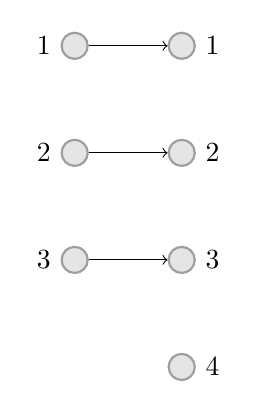
\begin{tikzpicture}[place/.style={circle,draw=darkgray!50,fill=gray!20,thick}]
       \node[place,label=left:1] (one3) {};
       \node[place,label=left:2] (two3) [below=of one3] {};
       \node[place,label=left:3] (three3) [below=of two3] {};

       \node[place,label=right:1] (one4) [right=of one3] {};
       \node[place,label=right:2] (two4) [below=of one4] {};
       \node[place,label=right:3] (three4) [below=of two4] {};
       \node[place,label=right:4] (four4) [below=of three4] {};

       \draw [->] (one3) to [thick, shorten <=1pt,>=stealth'] (one4);
       \draw [->] (two3) to [thick, shorten <=1pt,>=stealth']  (two4);
       \draw [->] (three3) to [thick, shorten <=1pt,>=stealth']  (three4);
    \end{tikzpicture}}
\hspace{7.5em}
  \subfigure[]{
  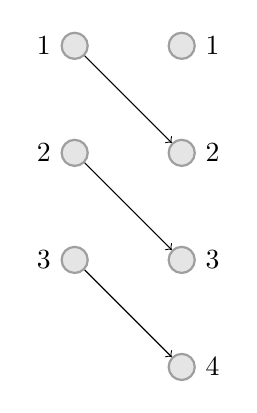
\begin{tikzpicture} [place/.style={circle,draw=darkgray!50,fill=gray!20,thick}]
       \node[place,label=left:1] (one3) {};
       \node[place,label=left:2] (two3) [below=of one3] {};
       \node[place,label=left:3] (three3) [below=of two3] {};

       \node[place,label=right:1] (one4) [right=of one3] {};
       \node[place,label=right:2] (two4) [below=of one4] {};
       \node[place,label=right:3] (three4) [below=of two4] {};
       \node[place,label=right:4] (four4) [below=of three4] {};

       \draw [->] (one3) to [thick, shorten <=1pt,>=stealth'] (two4);
       \draw [->] (two3) to [thick, shorten <=1pt,>=stealth']  (three4);
       \draw [->] (three3) to [thick, shorten <=1pt,>=stealth']  (four4);
  \end{tikzpicture}}

\vspace{4ex}
\caption{The graph of the |inject| function (a) and the |raise|
  function (b) embedding |Fin 3| in |Fin (3 + 1)|}
  \label{fig:fins}
\end{figure}

Using |inject| and |raise| as defined to work on finite sets, we can
define similar functions that work on our |Rule| and |Term| data
types.



\subsection{Proof search}

Our implementation of proof search is divided up into two steps.
In the first step we set up an abstract representation of the search
space in which we implement the basic machinery of sequential rule
application.
In the second step we transform this abstract representation into a
concrete search tree by branching over a set of rules.

The reason we have chosen to separate these two steps is that it
neatly separates the machinery for proof search (be it breath-first
search, depth-first search or some heuristic-driven algorithm) from
the machinery for unification.

Below we wil discuss both steps in turn.

\subsubsection*{Setting up the search space}

First off, let us discuss the data type that we will use to model the
abstract search space.

\begin{code}
  data SearchSpace (m : ℕ) : Set where
    done  : (∃₂ δ n → Subst (m + δ) n) → SearchSpace m
    step  : (∃ Rule → ∞ (SearchSpace m)) → SearchSpace m
\end{code}

In the above definition, |m| will denote the number of variables in
the goal; $\delta$ will denote the number of space that is needed for
rule application; and |n| will denote the number of variables
remaining after substitution. In fact, this naming is consistent, and
will also apply to further definitions.

The |done| constructor can then be read as returning a ``substitution
over terms with at least |m| free variables, which results a term with
|n| free variables when applied.''

The |step| constructor is what makes the representation abstract; it
provides a function that, when given any rule, will tell you how that
rule furthers the search.

\pepijn{Shall we use standard ``musical'' notation for coinductives?}

We then define a function |solve| that will be in charge of building
up an instance of |SearchSpace| from a goal, with the following
signature.

\pepijn{The following code will not actually compile, since we need to
rewrite with a proof that $(x + 0) = x$; but this definition is clearer.}

\begin{code}
  solve : ∀ {m} → (goal : Term m) → SearchSpace m
  solve {m} g = solveAcc {m} {0} (just (m , nil)) (g ∷ [])
\end{code}

The |solve| function is once again defined by an helper function with
an accumulating parameter, this time accumulating partial
substitutions while attempting to solve a list of (sub)goals.

\begin{code}
  solveAcc  : ∀ {m δ₁} → Maybe (∃ (λ n → Subst (m + δ₁) n))
            → List (Goal (m + δ₁)) → SearchSpace m
  solveAcc {m} {δ₁}  (just (n , s))  []        = done (δ₁ , n , s)
  solveAcc {m} {δ₁}  nothing         _         = loop
  solveAcc {m} {δ₁}  (just (n , s))  (g ∷ gs)  = step next
\end{code}

If we have solved all sub-goals, we can simply return our
accumulating parameter, wrapped in a |done|.

However, if at any point the chosen rule is not unifiable with the
current sub-goal, the search space will resort to just looping. We will
see this below.

\begin{code}
  loop : ∀ {m} → SearchSpace m
  loop = step (λ _ → ~ loop)
\end{code}

And last, but not least, the interesting case. If we still have goals
to solve, and have not yet failed, we must recursively construct a new
|SearchSpace| (note that |next| is defined within the scope of
|solveAcc|).

For a given rule |r|, we compute the most general unifier of the
conclusion of |r| and our first sub-goal, prepend |r|'s premises to
the list of sub-goals, and continue our search from there.

There are a few details to note here.
First of all, note that we pass any existing substitutions to
|unifyAcc| as its accumulating parameter. This ensures that they are
applied before computing any new unifiers, and that they are passed on
to the resulting modifier.

Next, there is the problem of variables. We can only unify two terms
that are built up over the same set of variables. Therefore we must
ensure that the goal, the rule's conclusion and its premises share a
common set of variables.
However, if we want the resulting substitution to have any meaning, we
would like the variables used in the initial goal term to remain the
same. This is where |inject| and |raise| come in.

Recall that injecting a variable into a larger set would keep its
value the same, whereas raising would raise the variable into the
portion of the set that was previously inaccessible. Therefore we will
always take care to |inject| our goal terms, and our accumulating
substitution, whereas we will |raise| the terms in the applied
rule.

Note that $\delta_2$ (the number of free variables in the chosen rule)
is added to $\delta_1$ (the amount of space that had to be made for
previous rule applications). This means that the amount of space to be
made will grow throughout the proof search.

\begin{code}
  next : ∃ Rule → ∞ (SearchSpace m)
  next (δ₂ , r) = ~ solveAcc {m} {δ₁ + δ₂} mgu (prm′ ++ gs′)
    where
      mgu   : Maybe (∃ (λ n → Subst (m + (δ₁ + δ₂)) n))
      mgu   = unifyAcc g′ cnc′ s′
        where
          g′    : Term (m + (δ₁ + δ₂))
          g′    = injectTerm δ₂ g

          s′    : ∃ (Subst (m + (δ₁ + δ₂)))
          s′    = n + δ₂ , injectSubst δ₂ s

          cnc′  : Term (m + (δ₁ + δ₂))
          cnc′  = raiseTerm (m + δ₁) (conclusion r)

      gs′   : List (Term (m + (δ₁ + δ₂)))
      gs′   = injectTermList δ₂ gs

      prm′  : List (Term (m + (δ₁ + δ₂)))
      prm′  = raiseTermList (m + δ₁) (premises r)
\end{code}

\subsubsection*{Constructing search trees}

The second step in our proof search implementation is to transform the
|SearchSpace| we have just constructed into an N-ary search tree. We
do this by branching once for every rule, at every |step| constructor.
In addition to this, we maintain a trace of the used rules.

The result is expressed in terms of the following data type.

\begin{code}
data SearchTree (A : Set) : Set where
  fail  : SearchTree A
  retn  : A → SearchTree A
  fork  : ∞ (List (SearchTree A)) → SearchTree A
\end{code}

Where in our case, the type |A| becomes a tuple containing the
substitution that was our previous result, together a list of
rules. In order to keep the code readable, let us introduce the
following alias.

\begin{code}
  Result m = ∃₂ (λ δ n → Subst (m + δ) n) × Rules
\end{code}

The function that takes care of the transformation is almost
trivial. For a given set of rules, we simply traverse the
|SearchSpace| structure, where at every |step| we apply the
continuation to every rule.

\begin{code}
mkTree : ∀ {m} → Rules → SearchSpace m → SearchTree (Result m)
mkTree rs₀ s = mkTreeAcc rs₀ s []
\end{code}

The |mkTree| function is defined using an helper with an accumulating
parameter, which keeps track of the applied rules.

\begin{code}
mkTreeAcc : ∀ {m} → Rules → SearchSpace m → Rules → SearchTree (Result m)
mkTreeAcc rs₀ (done s)  ap  = retn (s , ap)
mkTreeAcc rs₀ (step f)  ap  =
  fork (~ map (λ r → mkTreeAcc rs₀ (! f r) (ap ∷ʳ r)) rs₀)
\end{code}

After the transformation, we are left with a simple tree structure,
for which we can define simple traversal strategies, such as
depth-first search (shown below) or breadth-first search (not shown,
but implemented).

\begin{code}
  dfs : ∀ {A} (depth : ℕ) → SearchTree A → List A
  dfs  zero    _          = []
  dfs (suc k)  fail       = []
  dfs (suc k)  (retn x)   = return x
  dfs (suc k)  (fork xs)  = concatMap (dfs k) (! xs)
\end{code}

Putting it all together, we can define a function |searchToDepth|,
which implements proof search up to a given depth |d|, i.e.\ it
constructs the |SearchSpace|, converts it to a |SearchTree|, and
searches this tree (in this case using |dfs|) up to depth |d|.

\begin{code}
searchToDepth : ∀ {m} → ℕ → Rules → Goal m → List (Result m)
searchToDepth depth rules goal =
  dfs depth (mkTree rules (solve goal))
\end{code}

\pepijn{I have never introduced the goal type... and somewhere above I
use (goal : Term m), but I think that using Goal is less
verbose... though maybe somewhat less clear... I can also just go for
using Term... any thoughts?}


\section{Constructing proof trees}
\label{sec:proofs}

In the previous section we have discussed the implementation of proof
search, returning a substitution which, when applied to the goal, will
provide the user with a variable-free term \pepijn{shoul probably
  change or remove this bit}.

Another piece of information which was returned by the proof search
was a trace of the applied rules. In the following section we will
discuss using this information to reconstruct the proof terms. That
is, we will construct terms of the following type. That is, the type
of closed terms.

\begin{code}
data ProofTerm : Set where
  con : RuleName → List ProofTerm → ProofTerm
\end{code}

Since we know the arities of the rules, the algorithm for
reconstructing these terms is simple.

We start from the back of the trace. Our invariant is that the trace
corresponds to a valid proof, and thus we know that the last rule
\emph{must} have an arity of zero. And thus we can safely turn it into
a proof term with an empty argument list.

We continue with the next-to-last argument, knowing that it may be a
rule with either an arity of zero (in which case we add it to the list
of proof terms) or an arity of one (in which case we give it the
proof term generated in the previous step as an argument).

The algorithm continues in this fashion until all we reach the first
rule in the trace, at which point our invariant states that our list
should contain exactly one element.

A downside of our current implementation is that we do not explicitly
encode this invariant, and thus we cannot define the proof term
construction as a total function. The case in the |toProofTerms|
function that cannot occur is marked with a comment, and our top-level
|toProofTerm| function is forced to return a |Maybe| value. This is
not a great downside as, due to the undecidability of first-order
proof search in general, we would have had to return a |Maybe| value
in any case \pepijn{should get rid of the term maybe-value; write an
incomplete/non-total function?}.

\begin{code}
toProofTerms : Rules → List ProofTerm
toProofTerms = foldr next []
  where
    next : ∃ Rule → List ProofTerm → List ProofTerm
    next (δ , r) pfs with arity r ≤? length pfs
    ... | no   r>p = [] -- should not occur
    ... | yes  r≤p =
      con (name r) (take (arity r) pfs) ∷ drop (arity r) pfs
\end{code}

\begin{code}
toProofTerm : Rules → Maybe ProofTerm
toProofTerm rs with toProofTerms rs
... | []     = nothing
... | p ∷ _  = just p
\end{code}


\section{Adding reflection}
\label{sec:reflection}


\section{Extended example}
\label{sec:example}

\todo{Give a bigger example of debugging/automated proving}

\section{Discussion}
\label{sec:discussion}

\pepijn{One ``problem'' with our current implementation of proof
  search is that, while we encode the maximum number of variables used
  in a term, we do not enforce that all variables are used. As a
  consequence of this, we cannot guarantee that the substitution
  obtained from a successful proof search will substitute \emph{all}
  variables. Since we don't actually \emph{use} the substitution
  though, this does not really bother use in using our Prolog library
  to define an |auto| tactic.}

\todo{Mention Idris}

Future work: auto rewrite; setoid rewrite; proof combinators.

limitations of using recursion in hint data base

Cf Agsy



Combining hint data bases (\pepijn{It's called ``concatenation'', use
  $\_\plus\_$ :)})

Debugging failed auto attempts, or other examples from
\url{http://adam.chlipala.net/cpdt/html/LogicProg.html}

We cannot `insert goals' in the term produced by a call to auto. This
could be useful if you want to allow a tactic to return an unfinished
proof. Or can we? \pepijn{Nope? I'm afraid I still don't understand
the concept of |auto| generating existentials (or |iauto|?).}

Work with \emph{typed} term language. This is a hard problem.

Compare with Mtac.

Cite Devriese paper.

\bibliographystyle{plainnat}
\bibliography{main}

\end{document}

%%% Local Variables:
%%% mode: latex
%%% TeX-master: t
%%% TeX-command-default: "rake"
%%% End:
